\documentclass[authorproof,JRM,paper]{fujipressarticle}
\usepackage{graphicx}
\usepackage{cite}

%\usepackage{luatexja-preset}%日本語を使う場合。
%\ltjsetparameter{jacharrange={-2,-3}}

\usepackage[resetlabels,labeled]{multibib}%Using BibTeX
\newcites{Online}{Supporting Online Materials:}

%%% following commands are unnecessary to edit %%%
\setcounter{page}{1}
\SetVolume{00}
\SetIssueNo{0}
\SetPubYear{0000}
%\SetArticleID{Rb00-0-0000}
%%%%%%%%%%%%%%%%%%%%%%%%%%%%%%%%%%%%%%%%%%%%%%%%%%

\begin{document}

\pagestyle{fujipressstyle}

\title{Title of Your Paper}
\author{Your Name(s)}
\address{Your Institute(s)\\
	Address(es) of Your Institute\\
	E-mail: Your E-mail address(es)}
\markboth{Your Name(s)}{(Short) Title of Your Paper}
\dates{2000/00/00}{2000/00/00}
\maketitle


\begin{abstract}% Do not delete this percent symbol
	\noindent (Abstract) Please write down your abstract here without an indent.  The word ``Abstract'' is not needed.  
\end{abstract}

\begin{keywords}
	keyword1, keyword2, keyword3, .. (up to five)
\end{keywords}


\section{Section}
An example of an equation.

\begin{equation}
	i \hbar \frac{\partial \psi (x,t)}{\partial  t} = -\frac{\hbar ^2}{2m}{\nabla}^2 \psi (x,t)
\end{equation}\par
~\par
If you need to use bold face in equations, please use the \verb|\boldsymbol{x}| command,
\begin{equation}
	i \hbar \frac{\partial \psi (\boldsymbol{x},t)}{\partial  t} = -\frac{\hbar ^2}{2m}\boldsymbol{{\nabla}}^2 \psi (\boldsymbol{x},t)
\end{equation}


Regarding percentage, degree, minute, and second signs, no space between the numeral and the sign is needed, as par to the “closed style” used in American English format.\par
  Percentage sign: ~~10\%\par
  Degree sign: ~~~~~~~~10°C\par
  Geographic coordinates: ~~N 35°21'14" \par


\section{Section}
\subsection{Sub-Section}
Sub-Section 2-1.\cite{jrm:86}

\subsubsection{Sub-Sub-Section}
Sub-Sub-Section 2-2-1.\citeOnline{jrm:24}

\acknowledgments
Acknowledgments.

\begin{table}[t]
	\begin{center}
		\caption{Caption of table.}
		\label{table}
		\renewcommand{\arraystretch}{1.5}
		\begin{tabular}{|c|c|c|c|c|}
			\hline
			\textbf{Variable} & \textbf{N} & \textbf{Mean}& 
			\textbf{Max} & \textbf{Min}  \\ \hline
			A & 10& 50& 100& 0  \\ \hline
			B & 20& 80& 200& 0  \\ \hline
		\end{tabular}
	\end{center}
\end{table}

\begin{figure}[t]
	\centering
	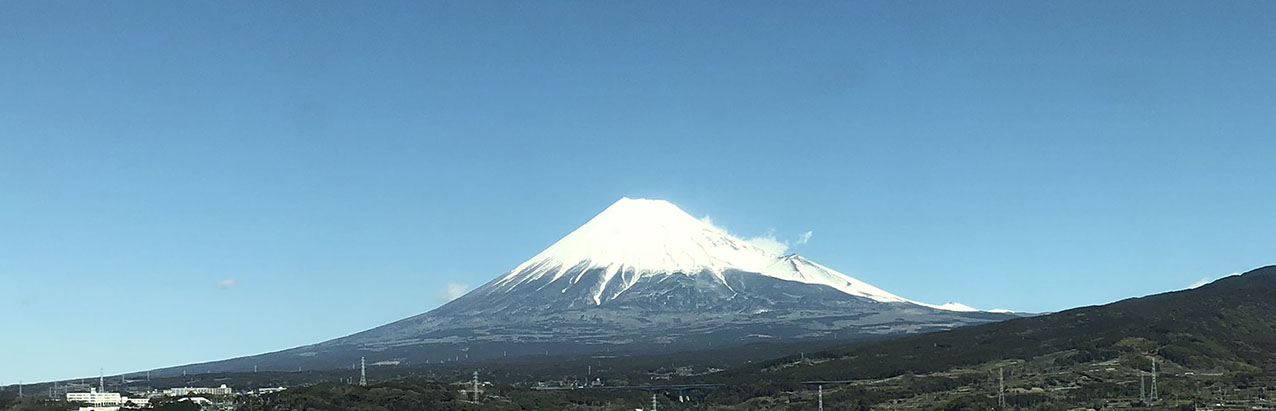
\includegraphics[width=8cm]{./fig/fig.jpg}
	\caption{Caption for fig.}
	\label{fig}
\end{figure}


\bibliographystyle{fujipressbib}%if you use bibtex
\bibliography{refdata}

\bibliographystyleOnline{fujipressbib}
\bibliographyOnline{refdata}



\appendix
\section{App-Section}
Appendix A.


%*Profiles and photos are not necessarily required at the first submission
\begin{profile}
	\Name{Your Name}
	\Orcid{0000-0000-0000-0000}
	\Affiliation{Your Institute}
	\Address{Address of Your Institute}
	\History{Your History}
	\Works{$\bullet$ Your Works}
	\Membership{$\bullet$ Your Academic and/or Learned Societies}
	%%please place any image files in subdirectory named ``fig''
	\Photo{./fig/photosample.pdf}
\end{profile}


\end{document}
